%%%%%%%%%%%%%%%%%%%%%%%%%%%%%%%%%%%%%%%%%%%%%%%%%%%%%%%%%%%%%%%%%%%%%%%%%%%%%%%%
%2345678901234567890123456789012345678901234567890123456789012345678901234567890
%        1         2         3         4         5         6         7         8

\documentclass[letterpaper, 10 pt, conference]{ieeeconf}  % Comment this line out
                                                          % if you need a4paper
%\documentclass[a4paper, 10pt, conference]{ieeeconf}      % Use this line for a4
                                                          % paper

\IEEEoverridecommandlockouts                              % This command is only
                                                          % needed if you want to
                                                          % use the \thanks command
                                                          \usepackage[utf8]{inputenc}
\usepackage[utf8]{inputenc}
\overrideIEEEmargins
% See the \addtolength command later in the file to balance the column lengths
% on the last page of the document



% The following packages can be found on http:\\www.ctan.org
%\usepackage{graphics} % for pdf, bitmapped graphics files
%\usepackage{epsfig} % for postscript graphics files
%\usepackage{mathptmx} % assumes new font selection scheme installed
%\usepackage{times} % assumes new font selection scheme installed
\usepackage{amsmath} % assumes amsmath package installed
\usepackage{amssymb}  % assumes amsmath package installed
\usepackage{fancyhdr}
\setlength{\headheight}{15.2pt}
\usepackage[]{algorithm2e}
\usepackage{url}
\usepackage{graphicx}
\usepackage{float}

\newtheorem{thm}{Theorem}
\newtheorem{lem}{Lemma}
\newtheorem{defi}{Definition}
\newtheorem{prop}{Proposition}
\newtheorem{conj}{Conjecture}

\DeclareMathOperator*{\ch}{ch}

% https://tex.stackexchange.com/questions/82271/multiple-algorithm2e-algorithms-in-two-column-documents
\makeatletter
\newcommand{\removelatexerror}{\let\@latex@error\@gobble}
\makeatother

\title{\LARGE \bf
%modif
On the list coloring of 1-band buffering cellular graphs
}

%\author{ \parbox{3 in}{\centering Huibert Kwakernaak*
%         \thanks{*Use the $\backslash$thanks command to put information here}\\
%         Faculty of Electrical Engineering, Mathematics and Computer Science\\
%         University of Twente\\
%         7500 AE Enschede, The Netherlands\\
%         {\tt\small h.kwakernaak@autsubmit.com}}
%         \hspace*{ 0.5 in}
%         \parbox{3 in}{ \centering Pradeep Misra**
%         \thanks{**The footnote marks may be inserted manually}\\
%        Department of Electrical Engineering \\
%         Wright State University\\
%         Dayton, OH 45435, USA\\
%         {\tt\small pmisra@cs.wright.edu}}
%}

\author{Marine Collery$^{1}$ and Benjámin Martin Seregi$^{2}$% <-this % stops a space
% \thanks{*This work was not supported by any organization}% <-this % stops a space
\thanks{$^{1}$ student of Research Methodology and Scientific Writing Course at KTH Kista P1P22017. e-mail: collery@kth.se}%
\thanks{$^{2}$ student of Research Methodology and Scientific Writing Course at KTH Kista P1P22017. e-mail: seregi@kth.se}%
}

\begin{document}


\maketitle
\thispagestyle{fancy}
\fancyhf{}
\chead{KTH Royal Institute of Technology | II2202, Fall 2017, Period 1-2 | \today}

\begin{abstract}
The optimal channel allocation problem in cellular networks is often formulated in a graph theoretic framework. One of its variants\---where each access point knows the list of its free channels\---is related the so-called list coloring problem. In spite of the fact that the list coloring problem is NP-complete for arbitrary graphs, we show that there exists a polynomial time algorithm for 1-band buffering callular graphs; and as a corollary it turns out the choice number of such a graphs is at most 4. In addition, we carry out performance comparisons between the existing integer linear programming solution and our implementation.
%%%%%% TODO Add statement about what the performance comparisons show. %%%%%% TODO
\end{abstract}

\begin{keywords}
channel allocation problem, cellular graph, list-coloring, choice number
\end{keywords}

%%%%%%%%%%%%%%%%%%%%%%%%%%%%%%%%%%%%%%%%%%%%%%%%%%%%%%%%%%%%%%%%%%%%%%%%%%%%%%%%
\section{Introduction}
%% TODO Since the available ... fix this
In telecommunication one of the most challenging problems is the efficient allocation of available frequency. Since the available bandwidth is usually limited (and expensive), the efficient utilization of the frequency spectrum is a major concern. Due to the growing number of mobile Internet users, the optimal channel allocation in cellular networks and their variants have been heavily researched in recent years \cite{Audhya:2011:SCA:1988563.1988571}.

Several variants of the channel allocation problem have been defined based on the different channel constraints that a particular service might require. One of them is the so-called co-channel constraint where the same channel is not allowed to be assigned to neighboring cells simultaneously. This problem has been formalized as a graph coloring problem by many authors \cite{1456167}. Unfortunately, graph coloring is a well-known NP-complete problem \cite{Kar72} and therefore we do not know if a polynomial time algorithm for co-channel constraint satisfaction exists. Therefore various heuristic algorithms have been developed, the list of methods includes genetic algorithms, neural networks, graph-based, and other approaches \cite{Audhya:2011:SCA:1988563.1988571}.

Cellular network topologies are usually idealized as a certain geometric structure. The most common network structure is the hexagonal grid topology where each cell is represented by a regular hexagon (two cells are neighbors if they share a common boundary). In \cite{662943}, Sen, Roxborough, and Medidi exploited this special structure and proposed an algorithm that optimally solves the channel allocation problem in $k$-band buffering systems where $k$ is $1$ or $2$. Moreover, the algorithm has polynomial running time $O(p)$ where $p$ is the number of cells.

R. Wang, et al. \cite{7248845} introduced a \textit{distinctly different} channel allocation problem from all the above mentioned problems, by assuming a $2$-band buffering hexagonal cell topology (the interference graph created from this topology is called a cellular graph) where each cell has a fixed number of frequency channels (channels are either busy or free). They asked the following question: "\textit{What is smallest size of the set of free channels associated with the cells (nodes of the cellular graph) that can guarantee interference free channel assignment to all the nodes?}". This problem is related to one of the generalizations of the graph coloring problem, called list coloring. It turned out that the required number of free channels is between $8$ and $10$. In addition, two algorithms have been proposed to create an interference free assignment, that is, a list-coloring of the cellular graph. The first one is an integer linear programming formulation of the list coloring problem (and therefore it is not a polynomial algorithm), while the second one is a heuristic linear time algorithm that is, according to their experiment, within 12\% of the optimal solutions.

In Section \ref{sec:theoretical-framework}, we introduce the basic terms and notions that are required to understand the theory, this allows us to describe the problem in a graph theoretic setting in Section \ref{sec:problem-questions}. Our main goal is to reformulate the above-mentioned problem for \textit{$1$-band buffering cellular graphs}. Section \ref{sec:orientation} studies how to find an acyclic orientation of cellular graphs such that the indegree of the nodes are below some upper bound. In addition, we prove that this can be done in polynomial time. In Section \ref{sec:4-choosable}, we prove that cellular graphs are $4$-choosable. Section \ref{sec:dag} investigates how to find kernels in directed acyclic graphs in polynomial time. Section \ref{sec:4-list-coloring} combines all of the results of the previous sections and gives a polynomial time algorithm that constructs a $4$-list coloring of a cellular graph.

\section{Theoretical Framework}\label{sec:theoretical-framework}
In this section we introduce the basic notions and definitions that is essential to formulate the problem in a graph-theoretic setting.
\begin{defi} A graph $G$ is a  \textit{cellular graph} (see Fig. \ref{fig:cellular-graph}) if it is constructed from the hexagonal cell topology in the following way: each cell is a node and two nodes are connected if and only if they share a common boundary.
\end{defi}
\begin{figure}[!h]
\centering
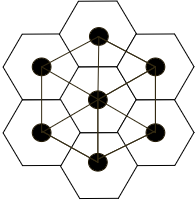
\includegraphics[scale=0.4]{cellular_graph.png}
\caption{An example of a cellular graph}\label{fig:cellular-graph}
\end{figure}
\begin{defi} A cellular network is $k$\textit{-band buffering} if the interference extends up to $k$ cells.
\end{defi}
\begin{defi} Let $G$ be a graph and $L(v)$ a set of colors for all $v \in V(G)$ such that $|L(v)|=k$. We say that $G$ is $k$\textit{-choosable} if $G$ is colorable such that the color of $v$ is in $L(v)$ for all $v \in V(G)$, such colorings called $k$\textit{-list coloring} of $G$.
\end{defi}
\begin{defi} The \textit{choice number} of $G$ is the smallest $k \in \mathbb{N}$ (notated by $\ch(G)$) such that $G$ is $k$-choosable.
\end{defi}

From now on we assume that all graphs are connected. We can do it without the loss of generality as all the algorithms and proofs can be repeated for each connected component of a graph.
\section{Research questions}\label{sec:problem-questions}
Let $G$ be a cellular graph of an $1$-band buffering cellular network. In our paper, we answer the following questions:
\begin{enumerate}
\item What is the choice number of $G$?
\item How can we find an orientation of $G$ such that the newly constructed directed graph $G'$ does not contain directed cycles such that $d^+(v) \leqslant 3$ ($d^+(v)$ is the indegree of $v$) for all $v \in V(G')$ in polynomial time of the size of $G'$?
\item Does there exist a polynomial time algorithm that finds a kernel in the graph $G'$, that is, an independent set $K \subseteq V(G)$ that satisfies the following: for each node $u \in V(G) \setminus K$ there is a node $v \in K$ such that $(u,v) \in E(G)$?
\end{enumerate}
%%%%%%%%%%%%%%%%%%%%%%%%%%%%%%%%%%%%%%%%%%%%%%%%%%%%%%%%%%%%%%%%%%%%%%%%%%%%%%%%
\section{Acyclic orientations of cellular graphs}\label{sec:orientation}

% rewrite this
Let $G$ be a cellular graph of an $1$-band buffering cellular network. Find an orientation of $G$ such that the newly constructed directed graph $G'$ does not contain directed cycles such that $d^+(v) \leqslant 3$ ($d^+(v)$ is the indegree of $v$) for all $v \in V(G')$ in polynomial time of the size of $G'$. Construct a polynomial time algorithm that finds a kernel graph in $G'$, that is, an independent set $K \subseteq V(G)$ that satisfies the following: for each node $u \in V(G) \setminus K$ there is a node $v \in K$ such that $(u,v) \in E(G)$.

%%%%%%%%%%%%%%%%%%%%%%%%%%%%%%%%%%%%%%%%%%%%%%%%%%%%%%%%%%%%%%%%%%%%%%%%%%%%%%%%

\begin{lem}\label{lem:degree-constraint}
Let $G$ be a cellular graph. Then $G$ has a node $v$ such that $\deg(v) \leqslant 3$.
\end{lem}

\begin{proof} Let us consider the planar drawing of the graph $G$ which corresponds to its hexagonal topology.
Let $v$ be any node of $G$ and we assign $(0,0)$ to this node. We assign coordinates to every node starting from node $v$ in the following way. If a node $w$ is to the north of node $v$ then the coordinates of node $w$ is equal to the coordinates of node $v$ plus $(0,1)$. We summarize this method in Fig. \ref{fig:assignment} according to the cardinal directions.
\begin{figure}[!h]
\centering
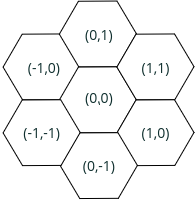
\includegraphics[scale=0.4]{hexagonal_coordinate_system.png}
\caption{Hexagonal coordinate system}\label{fig:assignment}
\end{figure}
By applying this method to every node, we get a coordinate system within our hexagonal topology. Since there are finitely many node in $V(G)$, we can select the maximal node by selecting the node with maximal $x$- and $y$-coordinate, that is, a node $w$ with the following property: if $(x_1,y_1)$ is the coordinates of $w$ and $v \neq w$ is another node with the coordinates $(x_2,y_2)$ then $x_1 \geqslant x_2$ and $y_1 > y_2$ are satisfied.

To obtain a contradiction, suppose that the maximal node $w$ has more than 3 neighbors. It follows then at least one if its neighbors is either to the north, northeast or southeast to $w$. However, this neighbor would violate the maximality of $w$. Therefore we proved that $\deg(w) \leqslant 3$.
\end{proof}
\begin{defi}
We say that the orientation of a digraph $G$ is $k$\textit{-bounded} if for each node $v \in V(G)$ its outdegree is bounded by $k$, that is, $\deg^+(v) \leqslant k$.
\end{defi}
\begin{lem}\label{lem:bounded-acyclic-orientation}
If $G$ is a cellular graph, then $G$ has a $3$-bounded acyclic orientation.
\end{lem}
\begin{proof} Since $G=(V,E)$ is a cellular graph, we can make use of Lemma \ref{lem:degree-constraint}, that is, let $v$ be a node of $G^{(0)}:=G$ with $\deg(v) \leqslant 3$. We construct a function $f\colon V(G) \to \mathbb{N}$ by setting $f(v) := 0$ and then remove the node $v$ from $G^{(0)}$ yielding the graph $G^{(1)}$. By repeating the same procedure - at step $i$th - we select a node $v$ in $G^{(i)}$ such that $\deg(v) \leqslant 3$ and we set $f(v):=i$. Then we remove $v$ from $G^{(i)}$ which yields the graph $V(G^{(i+1)}) := V(G^{(i)}) \setminus \lbrace v \rbrace$. It is trivial that the graphs $G^{(1)},\ldots,G^{(|V(G)|)}$ are all cellular therefore it was valid using Lemma \ref{lem:degree-constraint}.

We note that the procedure ends after $|V(G)|$ steps.

Now we construct a digraph $H=(V,A)$ from $G$ using the function $f$. Let $(u,v) \in E$ be an arbitrary edge. If $f(u) < f(v)$ then $A:=A\cup (u,v)$ otherwise $A:=A \cup (v,u)$. By repeating this procedure for all edges in $E$ we get an orientation of $G$, that is, the digraph $H$. We need to prove that $H$ is
\begin{enumerate}
\item acyclic and
\item $\deg^+(v) \leqslant 3$ holds for all $v \in V(G)$.
\end{enumerate}
To prove (1), we will obtain a contradiction by assuming that $H$ contains a directed cycle. Let $C$ be a directed cycle in $H$ with the nodes $C:=\lbrace v_1,v_2,\ldots,v_k \rbrace$ that are ordered such that $(v_i,v_{i+1 \bmod{k}}) \in E$ $(i=1,2,\ldots,k)$ which means that $f(v_1) < f(v_2) < \ldots < f(v_{k-1}) < f(v_k)$ but also $f(v_k) < f(v_1)$ which is impossible.

What is left to show is that $\deg^+(v) \leqslant 3$. At each step we select a node with no more than $3$ neighbors and those neighbors will be assigned a number that is greater than $f(v)$. Therefore the outdegree of $v$ cannot be larger than $3$.
\end{proof}

It is easy to see that the proof of this lemma can be transformed into a polynomial time algorithm. In what follows we outline the algorithm (Algorithm \ref{alg:find-acyclic-bounded-orientation}) that is based on the proof of Lemma \ref{lem:bounded-acyclic-orientation} and then we prove that its running time is $O(|V(G)| + |E(G)|)$.
\begin{algorithm}\label{alg:find-acyclic-bounded-orientation}
 \KwData{A cellular graph $G = (V,E)$}
 \KwResult{An acyclic $3$-bounded orientation of $G$}
 $G^{(0)} := G$\;
 Initialize $f \colon V(G) \to \mathbb{N}$\;
 \For{$i\leftarrow 0$ \KwTo $|V(G)|-1$}{
  Select $v \in V(G^i)$ such that $\deg(v) \leqslant 3$\;
  $f(v):=i$\;
  $V(G^{(i+1)}):=V(G^{i}) \setminus \lbrace v \rbrace$\;
 }
 Initialize $H:=(V,A)$\;
 \ForAll{$e = (u,v) \in E(G)$}{
   \eIf{$f(u) < f(v)$} {
   	$A := A \cup (u,v)$\;
   }{
   $A := A \cup (v,u)$\;
   }   
 }
 \caption{Constructing an acyclic $3$-bounded orientation of a cellular graph}
\end{algorithm}
\begin{prop} Algorithm \ref{alg:find-acyclic-bounded-orientation} has a running time of $O(|V(G)| + |E(G)|)$.
\end{prop}
\begin{proof}
It is enough to prove that "Select $v \in V(G^i)$ such that $\deg(v) \leqslant 3$" can be done in $O(|V(G)|)$ since the rest is obvious. Let us initialize a queue $Q := \lbrace v \mid \deg(v) \leqslant  3\rbrace$ before we start running the algorithm. We pop a node $v$ from $G$ at every iteration and push new ones after the removal of $v$ if there are new nodes in $G$ that satisfy the degree condition. The pop and push methods can be implemented in constant time which completes the proof.
\end{proof}

It is important to note that the idea of Algorithm \ref{alg:find-acyclic-bounded-orientation} came from \cite{CHROBAK1991243} where the authors proved that every planar graph has a $5$-bounded acyclic orientation. They used the fact that every planar graph has a node with at most $5$ neighbors which follows from Euler's formula.
\section{Cellular graphs are $4$-choosable}\label{sec:4-choosable}

We are about to prove one of our main results, that is, cellular graphs are $4$-choosable. We would like to note that since $G$ is a planar, it follows from Thomassen's theorem \cite{Thomassen:1994:PG:184180.184192} that it is $5$-choosable. It is worth noting that cellular graphs are $3$-colorable \cite{662943} (Theorem 1). However, even with this additional constraint, we still cannot say that if $G$ is planar and $3$-colorable then it is $4$-choosable as a counterexample can be found in \cite{JGT:JGT4}. The counterexample is quite interesting (\cite {JGT:JGT4}, second figure) as it is constructed from a cellular graph; however the author added one extra node and joined it to all of the outer nodes. Due to this step, the resulting graph does not always contain a node of degree $3$ therefore the property of Lemma \ref{lem:degree-constraint} is not true for this construction.

Before proving our theorem we need to introduce the notion of kernel in graphs and a theorem from Galvin \cite{Galvin:1995:LCI:199352.199369} (non-multigraph version from \cite{citeulike:395714}, Lemma 5.4.3) that will play a central role in our study. The proof of the theorem is inductive and can be transformed into an algorithm.
\begin{defi} Let $G$ be a directed graph. We say that an independent set $K \subseteq V(G)$ is a kernel of $G$ if it satisfies the following: for each node $u \in V(G) \setminus K$ there is a node $v \in K$ such that $(u,v) \in E(G)$.
\end{defi}
\begin{thm}[Galvin, 1995]\label{thm:galvin} Let $G$ be a graph and $\lbrace L(v) \mid v \in V(G) \rbrace$ given color sets. If $G$ has an orientation $D$ such that $d^+(v) < |L(v)|$ for all $v \in V(D)$ and every induced subgraph of $D$ has a kernel, then $G$ can be colored from the given color sets. $\blacksquare$
\end{thm}
We will reformulate this theorem later for cellular graphs. 
\begin{defi} We note that a directed graph is called kernel-perfect if all of its induced subgraphs contain a kernel.
\end{defi}
\begin{thm}\label{thm:choice-number}
If $G$ is a cellular graph then $\ch(G) \leqslant 4$.
\end{thm}
\begin{proof}
Since $G$ is cellular, we can consider its $3$-bounded acyclic orientation by Lemma \ref{lem:bounded-acyclic-orientation}. This orientation is kernel-perfect by Richardson's theorem \cite{richardson1946}. Therefore we can apply Theorem \ref{thm:galvin} (with $d^+(v) \leqslant 3$ and $L(v)=4$) which concludes the proof.
\end{proof}

We have proven that cellular graphs are $4$-choosable, hence what is left is to show that there exists an algorithm that constructs such colorings in polynomial time.
\section{Finding a kernel in DAGs}\label{sec:dag}

It has been shown that finding a kernel in an arbitrary graph is $\mathrm{NP}$-complete \cite{chvatal}. However, we will show that in directed acyclic graphs (DAGs) this problem can be easily solved in polynomial time. This is crucial as our $4$-list coloring algorithm has to construct kernels repeatedly at run.

\begin{lem}\label{lem:kernel-lemma} Let $G$ be a directed acyclic graph. Then a kernel $K \subseteq V(G)$ can be found in polynomial time.
\end{lem}
\begin{proof} Since $G$ is acyclic we can consider the topological order of its nodes (which can be computed in polynomial time). Let $\lbrace v_1, v_2, \ldots, v_n \rbrace$ be this topological order. Let us start from node $v_1$ and add it to the kernel, that is, $K = \lbrace v_1 \rbrace$. Mark the neighbors of $v_1$. After that, we move on with the second node $v_2$, if it is marked we skip it otherwise we add it to the kernel $(K := K \cup \lbrace v_2 \rbrace)$ and mark its neighbors. Repeat this procedure with the remaining nodes. We need to prove that
\begin{enumerate}
\item $K$ is independent and
\item for each node $u \in V(G) \setminus K$ there is a node $v \in K$ such that $(u,v) \in E(G)$.
\end{enumerate}
1) If $v \in K$ then its neighbors are marked. Since we do not add marked nodes to $K$, it is always independent.
2) When $v$ is unmarked and we add it to $K$ all of its neighbors come after it in the topological order (otherwise $v$ would have already been marked), that is, $v$ is connected to its neighbors by forward edges.
\end{proof}
\begin{algorithm}\label{alg:find-kernel-in-dags}
 \KwData{A directed acyclic graph $G = (V,A)$}
 \KwResult{A kernel $K \subseteq V(G)$}
 $T := \text{the topological order of $V(G)$}$\;
 $K := \emptyset$\;
 \For{$i\leftarrow 1$ \KwTo $|V(G)|$}{
  \If{$T(i)$ is unmarked} {
  	$K := K \cup \lbrace T(i) \rbrace$\;
  	Mark the neighbors of $T(i)$\;
  }
 }
 \caption{Finding a kernel in a DAG}
\end{algorithm}

We note that the topological order can be computed in linear time in the number of nodes and edges with Kahn's algorithm \cite{Kahn:1962:TSL:368996.369025}, therefore the running time of our algorithm is $O(|V(G)|+|E(G)|)$. We also note that an induced subgraph of a DAG is trivially a DAG, therefore from Algorithm \ref{alg:find-kernel-in-dags} it follows that DAGs are kernel-perfect, that is, there is no need to apply Richardson's theorem in the proof of Theorem \ref{thm:choice-number}.
\section{$4$-list coloring of cellular graphs}\label{sec:4-list-coloring}
Now we have everything necessary to prove our main result and give a polynomial algorithm that computes a $4$-list coloring of a cellular graph. 

First we reformulate Galvin's theorem for cellular graphs and prove it (Theorem \ref{thm:galvin}), the proof is based on \cite{citeulike:395714} (Lemma 5.4.3). The original proof uses mathematical induction, we just repeat the same argument, fortunately the inductive step describes how to color the nodes, that is, the proof can be transformed into an algorithm. The cellular version, however, uses our result, namely Lemma \ref{lem:bounded-acyclic-orientation}. In addition, it also uses Lemma \ref{lem:kernel-lemma}. Then we prove that its (Algorithm \ref{alg:four-list-coloring}) running time is polynomial. Algorithm \ref{alg:four-list-coloring} uses Algorithm \ref{alg:find-acyclic-bounded-orientation} and Algorithm \ref{alg:find-kernel-in-dags}. The fact that Algorithm \ref{alg:four-list-coloring} is polynomial follows from the fact that Algorithm \ref{alg:find-acyclic-bounded-orientation} and Algorithm \ref{alg:find-kernel-in-dags} are polynomial.
\begin{thm}[Galvin's theorem for cellular graphs] Let $G$ be a graph and $\lbrace L(v) \mid v \in V(G) \rbrace$ given color sets. If $G$ has a kernel-perfect orientation $D$ such that $d^+(v) < |L(v)|$ for all $v \in V(D)$, then $G$ can be colored from the given color sets.
In particular, if $G$ is a cellular graph and $|L(v)| \geqslant 4$ for all $v \in V(G)$. Then $G$ can be colored from the given color sets.
\end{thm}
\begin{proof}
Let $G^*$ be the $3$-bounded acyclic orientation of $G$ (Lemma \ref{lem:bounded-acyclic-orientation}), that is, $d^+(v) \leqslant 3$. We apply induction on $|V(G^*)|$. For $|V(G^*)|=0$, the empty coloring is good. Let us assume that we know how to color $G^*$ with $|V(G^*)| < n$ and consider the case when $|V(G^*)|=n$. Let $\alpha$ be any color from one of the colors sets and set $V_\alpha$ to $\lbrace v \in V(G) \mid \alpha \in L(v) \rbrace$. Consider the non-empty subgraph $D$ of $G^*$ that is spanned by $V_\alpha$. Since $G^*$ is a DAG, it is kernel-perfect (Lemma \ref{lem:kernel-lemma}), therefore $D$ has a kernel $U \neq \emptyset$. Assign the color $\alpha$ to every node in $U$ and remove $\alpha$ from $L(v)$ for all $v \in V_\alpha$. Since $U$ is independent, and we removed $\alpha$, it follows that we did not (and we will not) violate the rules of the graph coloring. After that, remove $U$ from $D$, since every node in $V(D) \setminus U$ sends an edge to $U$, having removed $U$ from $D$, we decreased the outdegree of each node in $D$ by $1$. Since the modified lists $L'(v)$ $(v \in V_\alpha)$ satisfy $d^+(v) < |L'(v)|$ for all $v \in V(D) \setminus U$, we can use our induction hypothesis to color $V(G^*) \setminus U$.
\end{proof}
\begin{figure}[H]
\removelatexerror
\begin{algorithm}[H]\label{alg:four-list-coloring}
 \KwData{A cellular graph $G$ and a set of colors $L(v)$ for all $v \in V(G)$ with $|L(v)| \geqslant 4$}
 \KwResult{$4$-list coloring of $G$}
  Let $G^*$ be the $3$-bounded acyclic orientation of $G$ (Algorithm \ref{alg:find-acyclic-bounded-orientation})\;
  \While{$V(G^*)$ is non-empty} {
  	Let $\alpha$ be a color from $L(v)$ where $v \in V(G^*)$\;
  	$V_\alpha := \lbrace v \in V(G) \mid \alpha \in L(v) \rbrace$\;
  	Let $D$ be the subgraph of $G^*$ that $V_\alpha$ spans\;
  	Let $U$ be a kernel in $D$ (Algorithm \ref{alg:find-kernel-in-dags})\;
  	Color the nodes in $U$ with color $\alpha$\;
  	Remove $\alpha$ from $L(v)$ for all $v \in V_\alpha$\;
  	Remove the colored nodes, that is, $V(G^*) := V(G^*) \setminus U$\;
  }
 \caption{$4$-list coloring of a cellular graph}
\end{algorithm}
\end{figure}
It can be seen from the algorithm that first we call Algorithm \ref{alg:find-acyclic-bounded-orientation} then we call Algorithm \ref{alg:find-kernel-in-dags} multiple times. If we assume the worst-case scenario when the kernel $U$ has only $1$ element, then the while loop iterates $|V(G)|$ times. The auxiliary operations such as spanning a subgraph or creating the set $V_\alpha$ can be done in linear time. Therefore the overall running time of our algorithm is $O(|V(G)|^2+|V(G)||E(G)|)$.

In each iteration, we color the nodes in $U$ and remove one color. The color is proper by Theorem \ref{alg:four-list-coloring}. However, we need to show that in each iteration every node is either colored or it has a free available color.
\begin{lem} Algorithm \ref{alg:four-list-coloring} is correct, that is, in each iteration every node is either colored or it has a free available color.
\end{lem}
\begin{proof} To obtain a contradiction, let us suppose that there is a node $v$ that is not colored and it does not have an available color ($|L(v)|=0$). This means that $v$ was in $V_{\alpha}$ for at least $4$ different colors and it was never in the kernel. However, this would mean that $d^+(v) \geqslant 4$ as $v$ sent an edge to each kernel. This is impossible since $G$ is $3$-bounded.
\end{proof}
\section{Methods}

Our method is analytical since the $1$-band buffering cellular topology can be easily modeled as a graph. In order to prove that our solution is optimal and fast we cannot use empirical methods as it would not cover all the possible topologies that might arise in network deployments.

\section{Results and Analysis}

\textit{All the code referenced below is open source and available here: \texttt{https://github.com/Benmartin92 /research-kth}. \\\\}

The algorithms are implemented in Java in order to test their correctness. The graphs are displayed in a JApplet in order to visualize the coloring. The implementation is based on the JGraphT \cite{JGraphT} libraries which provides the graph data structures.

\subsection{Generation of Cellular Graph}
The cellular graphs are generated from a grid graph shown in Fig. \ref{cellgraphgeneration}.

\begin{figure}[!h]
\centering
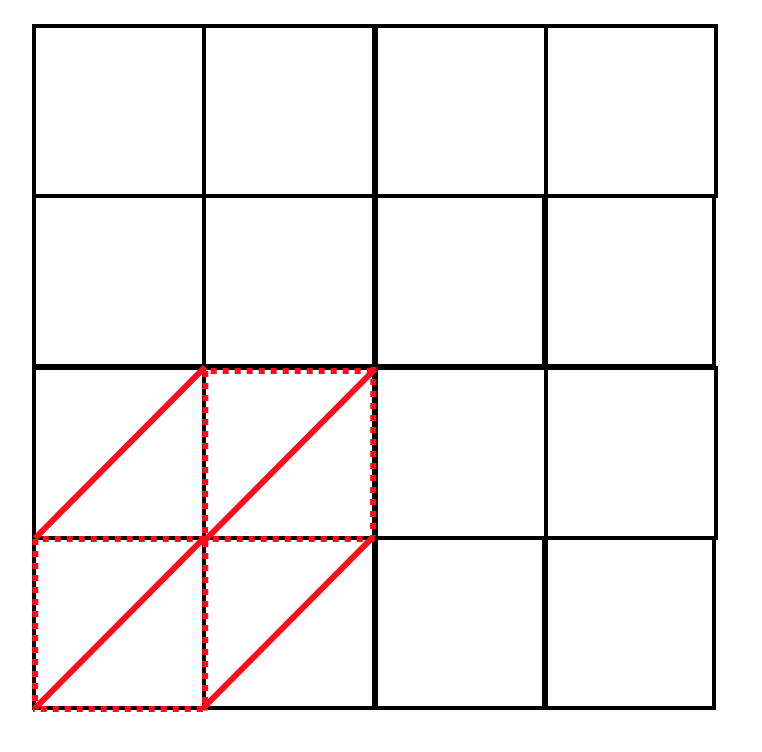
\includegraphics[scale=0.4]{cellGeneration.png}
\caption{Example of generation of one cell in a grid with $N=5$.}
\label{cellgraphgeneration}
\end{figure}

\subsection{Cellular Graph - 4 colors and each are available for each node}
The first observation that we could make is that only $3$ colors were used to color a cellular graph with no restrictions.

\begin{figure}[!h]
\centering
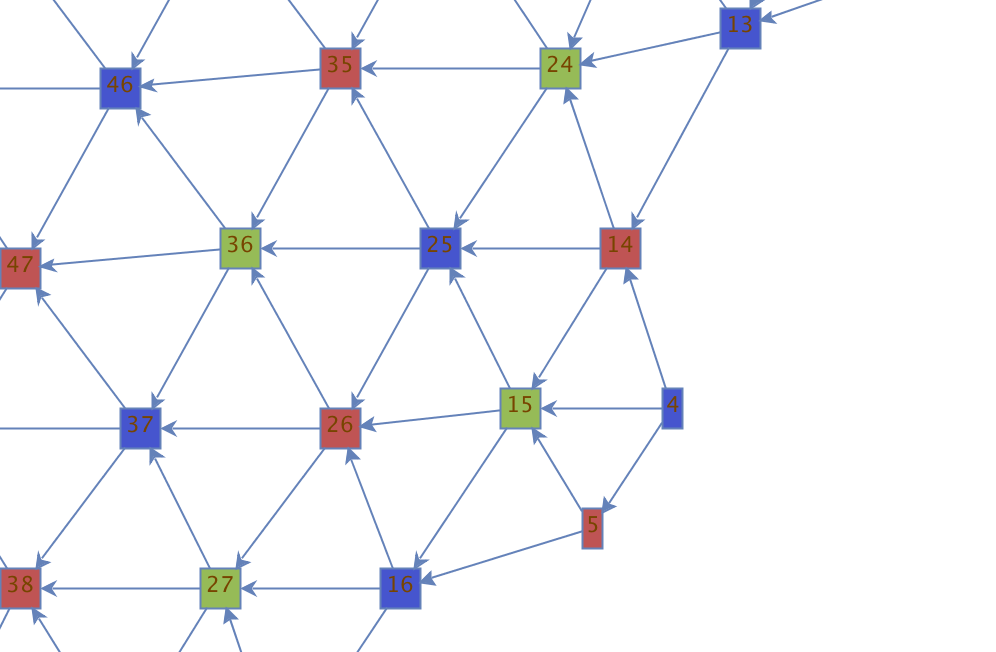
\includegraphics[scale=0.4]{3colors.png}
\caption{Example of a part of cellular graph colored.}
\end{figure}

We then studied the running time of the algorithm compared to an integer linear program from \cite{7248845} with cellular graphs of variable sizes.
The running time of the integer linear program solved by GLPK \cite{GLPK} is given in seconds while the running time of our implementation are in nanoseconds.
We can notice the exponential time required for the integer linear program compared to our polynomial one on Fig. \ref{4colors}

\begin{figure}[!h]
\centering
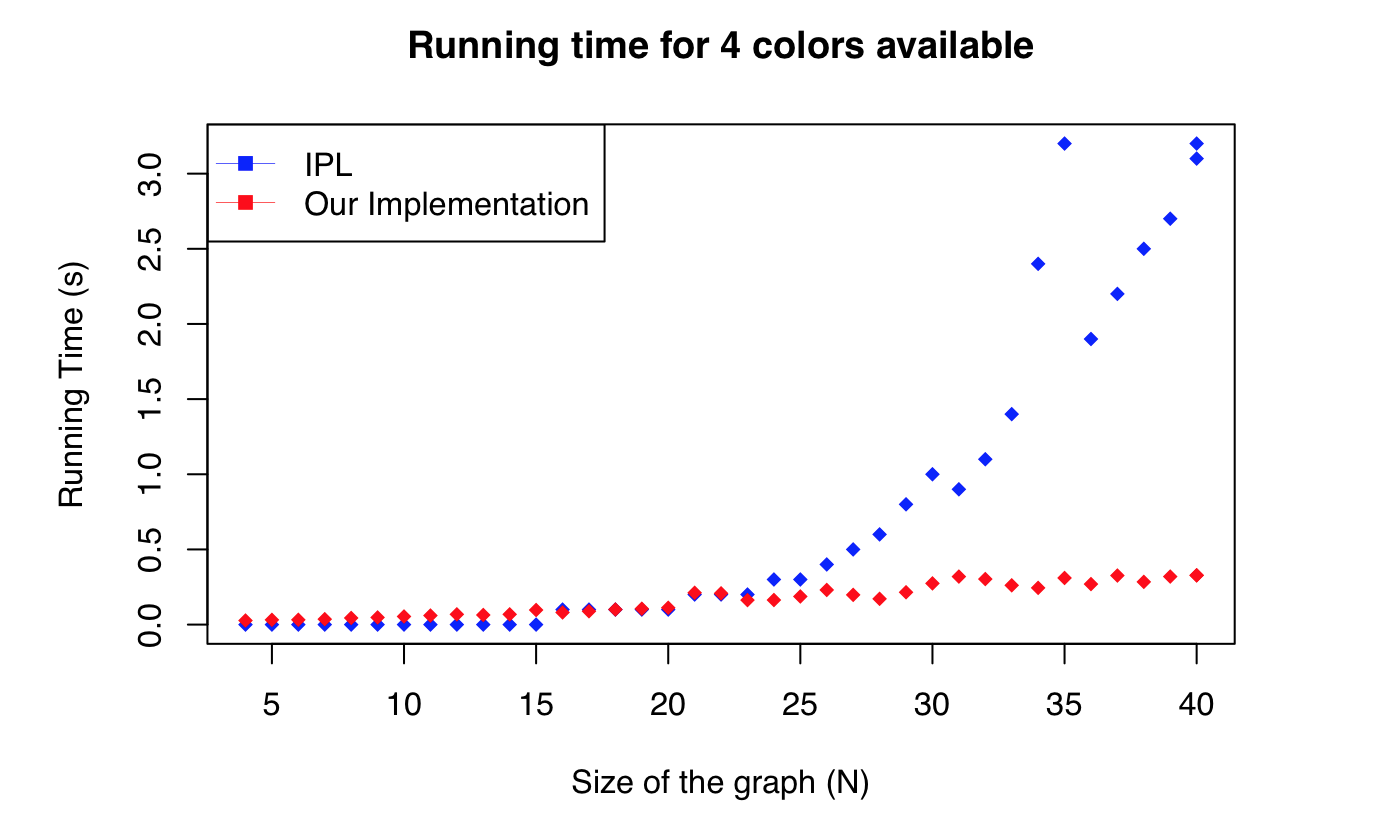
\includegraphics[scale=0.4]{4colorsRunTime.png}
\caption{R studio result.}
\label{4colors}
\end{figure}


\subsection{Cellular Graph - random numbers of colors available (higher than 4), each node has 4 possible colors}

The fact that the running time depends on the number of colors available for a fixed size of cellular graph is though to test. However, the running time of the integer linear program and its need in memory can be very high.
Cellular graphs with very few nodes have been tested because the physical requirements (CPU, memory) for higher numbers of nodes were not available.
Fig. \ref{20size} shows some value where the integer linear program gave a solution in less than $2$ minutes. We can see that when the integer linear program gives a solution fast then so does our algorithm.
No further conclusions can be made until we generate more data especially with larger cellular graphs.

\begin{figure}[!h]
\centering
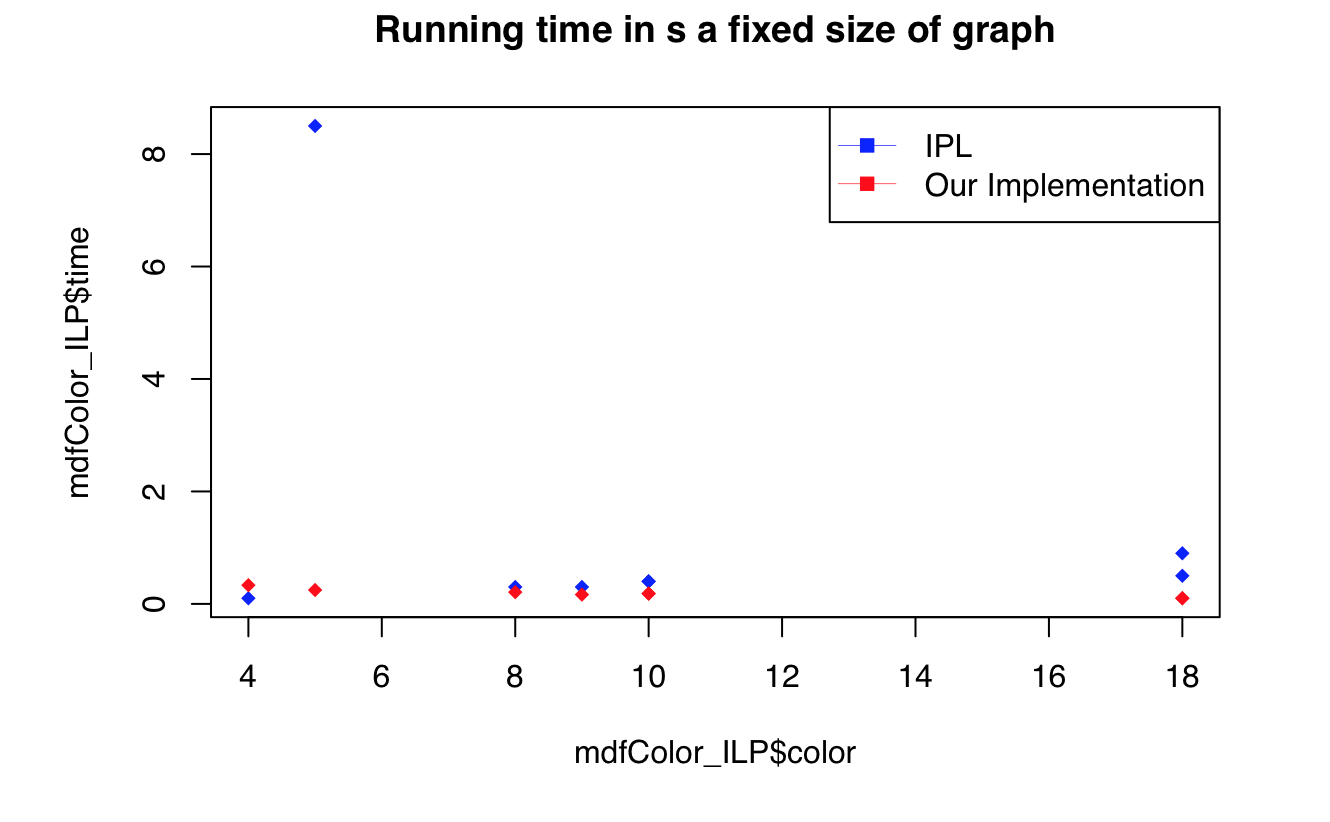
\includegraphics[scale=0.4]{20sizeRunTime.png}
\caption{R studio result for a fixed size of $N=20$ (cf.Fig.\ref{cellgraphgeneration})}
\label{20size}
\end{figure}


\section{Discussion}

We have proven that cellular graph are 4-choosable and this proposition has been tested in practice. We found that when the same $4$ colors are available at each node, the algorithm has colored the graph with only $3$ colors. This result verifies the fact that $1$-band buffering cellular graphs are $3$-colorable \cite{662943}.
The test showed that the running time of our implementation depends on the size of the cellular graph and it is lower than the integer linear program implementation especially for large cellular graphs.
Most of the work has been done comparing our algorithm to the integer linear program.
The next step in this project is to run extensive simulations with both of the implementations and compare the results.


\addtolength{\textheight}{-12cm}   % This command serves to balance the column lengths
                                  % on the last page of the document manually. It shortens
                                  % the textheight of the last page by a suitable amount.
                                  % This command does not take effect until the next page
                                  % so it should come on the page before the last. Make
                                  % sure that you do not shorten the textheight too much.

%%%%%%%%%%%%%%%%%%%%%%%%%%%%%%%%%%%%%%%%%%%%%%%%%%%%%%%%%%%%%%%%%%%%%%%

\bibliographystyle{IEEEtran}
\bibliography{ref.bib}
\end{document}